\chapter{System design}

In the previous chapter, we have extracted the functional and non-functional requirements of our system. Subsequently, we broke down our system into use cases in the Use Case Model [\ref{fig:UCM}]. Furthermore, we have described the entities of our system and the relationships between them using an Analysis Object Model [\ref{fig:AOM}].

In this chapter we map our analysis into the solution domain. We group the objects that we have identified in the Analysis Object Model [\ref{fig:AOM}] into subsystems. The implementation details of our subsystems and the dependencies between them are also discussed.

\section{Design Goals}

In the previous chapter we have defined our Non-functional requirements. In this chapter, we use those non-functional requirements to extract our design goals, and we use those design goals as a compass for our system design. Defining our design goals allows us make consistent design decisions accross our different subsystems. Table [\ref{tab:DG}] lists our non-functional requirements and their corresponding design goal. There are 5 types of possible design criteria from which the design goals can be selected: performance, dependability, cost, maintenance and end user criteria \cite{bruegge2004object}.

\begin{table}
  \centering
  \begin{tabular}{ | l | p{5cm} | l | }
    \hline
    \textbf{Requirement} & \textbf{Design Goal} & \textbf{Criteria} \\ \hline
    \textbf{Accuracy} & The system should be dynamic enough to accomodate the addition of new classes. & Performance \\ \hline
    \textbf{Adaptability} & The system should be able to classify different small parts with high accuracy. & Performance \\ \hline
  \end{tabular}
  \caption{Non-functional requirements and their corresponding design goals}
  \label{tab:DG}
\end{table}

\section{Subsystem Decomposition}

Figure [\ref{fig:SSD}] depicts the system's subsystem decomposition. Our system is divided into 3 subsytems: SyntheticImageServer, RealImageServer and ImageClassifier.

\subsection{SyntheticImageServer}
SyntheticImageServer is responsible for providing our system with synthetic images. It consists of 2 main components: SyntheticScene and SyntheticImageGenerator. The SyntheticScene generates an artificial environment and places a 3DModel inside said environment. The SyntheticImageGenerator renders 2D images of the 3D artificial scene.

\subsection{RealImageServer}
The RealImageServer is the SyntheticImageServer's counterpart. It is responsible for providing our system with real images. The RealImageGenerator uses the Camera to take real images of the small parts. Next, the RealImageGenerator performs some processing on the raw images to provide our system with real images that can be used out of the box.

\subsection{ImageClassifier}
ImageClassifier consumes both the real and syntheic images, and stores them in a Dataset. The images are then fed to the DataSplitGenerator, which is in turn responsible for splitting the data into a training set, a validation set and a testing set.

The CNNModel consumes the training set and the validation set to utilize them during the training phase. The testing set is then used to determine the accuracy of the trained CNNModel.

\begin{figure}[H]
\centering
  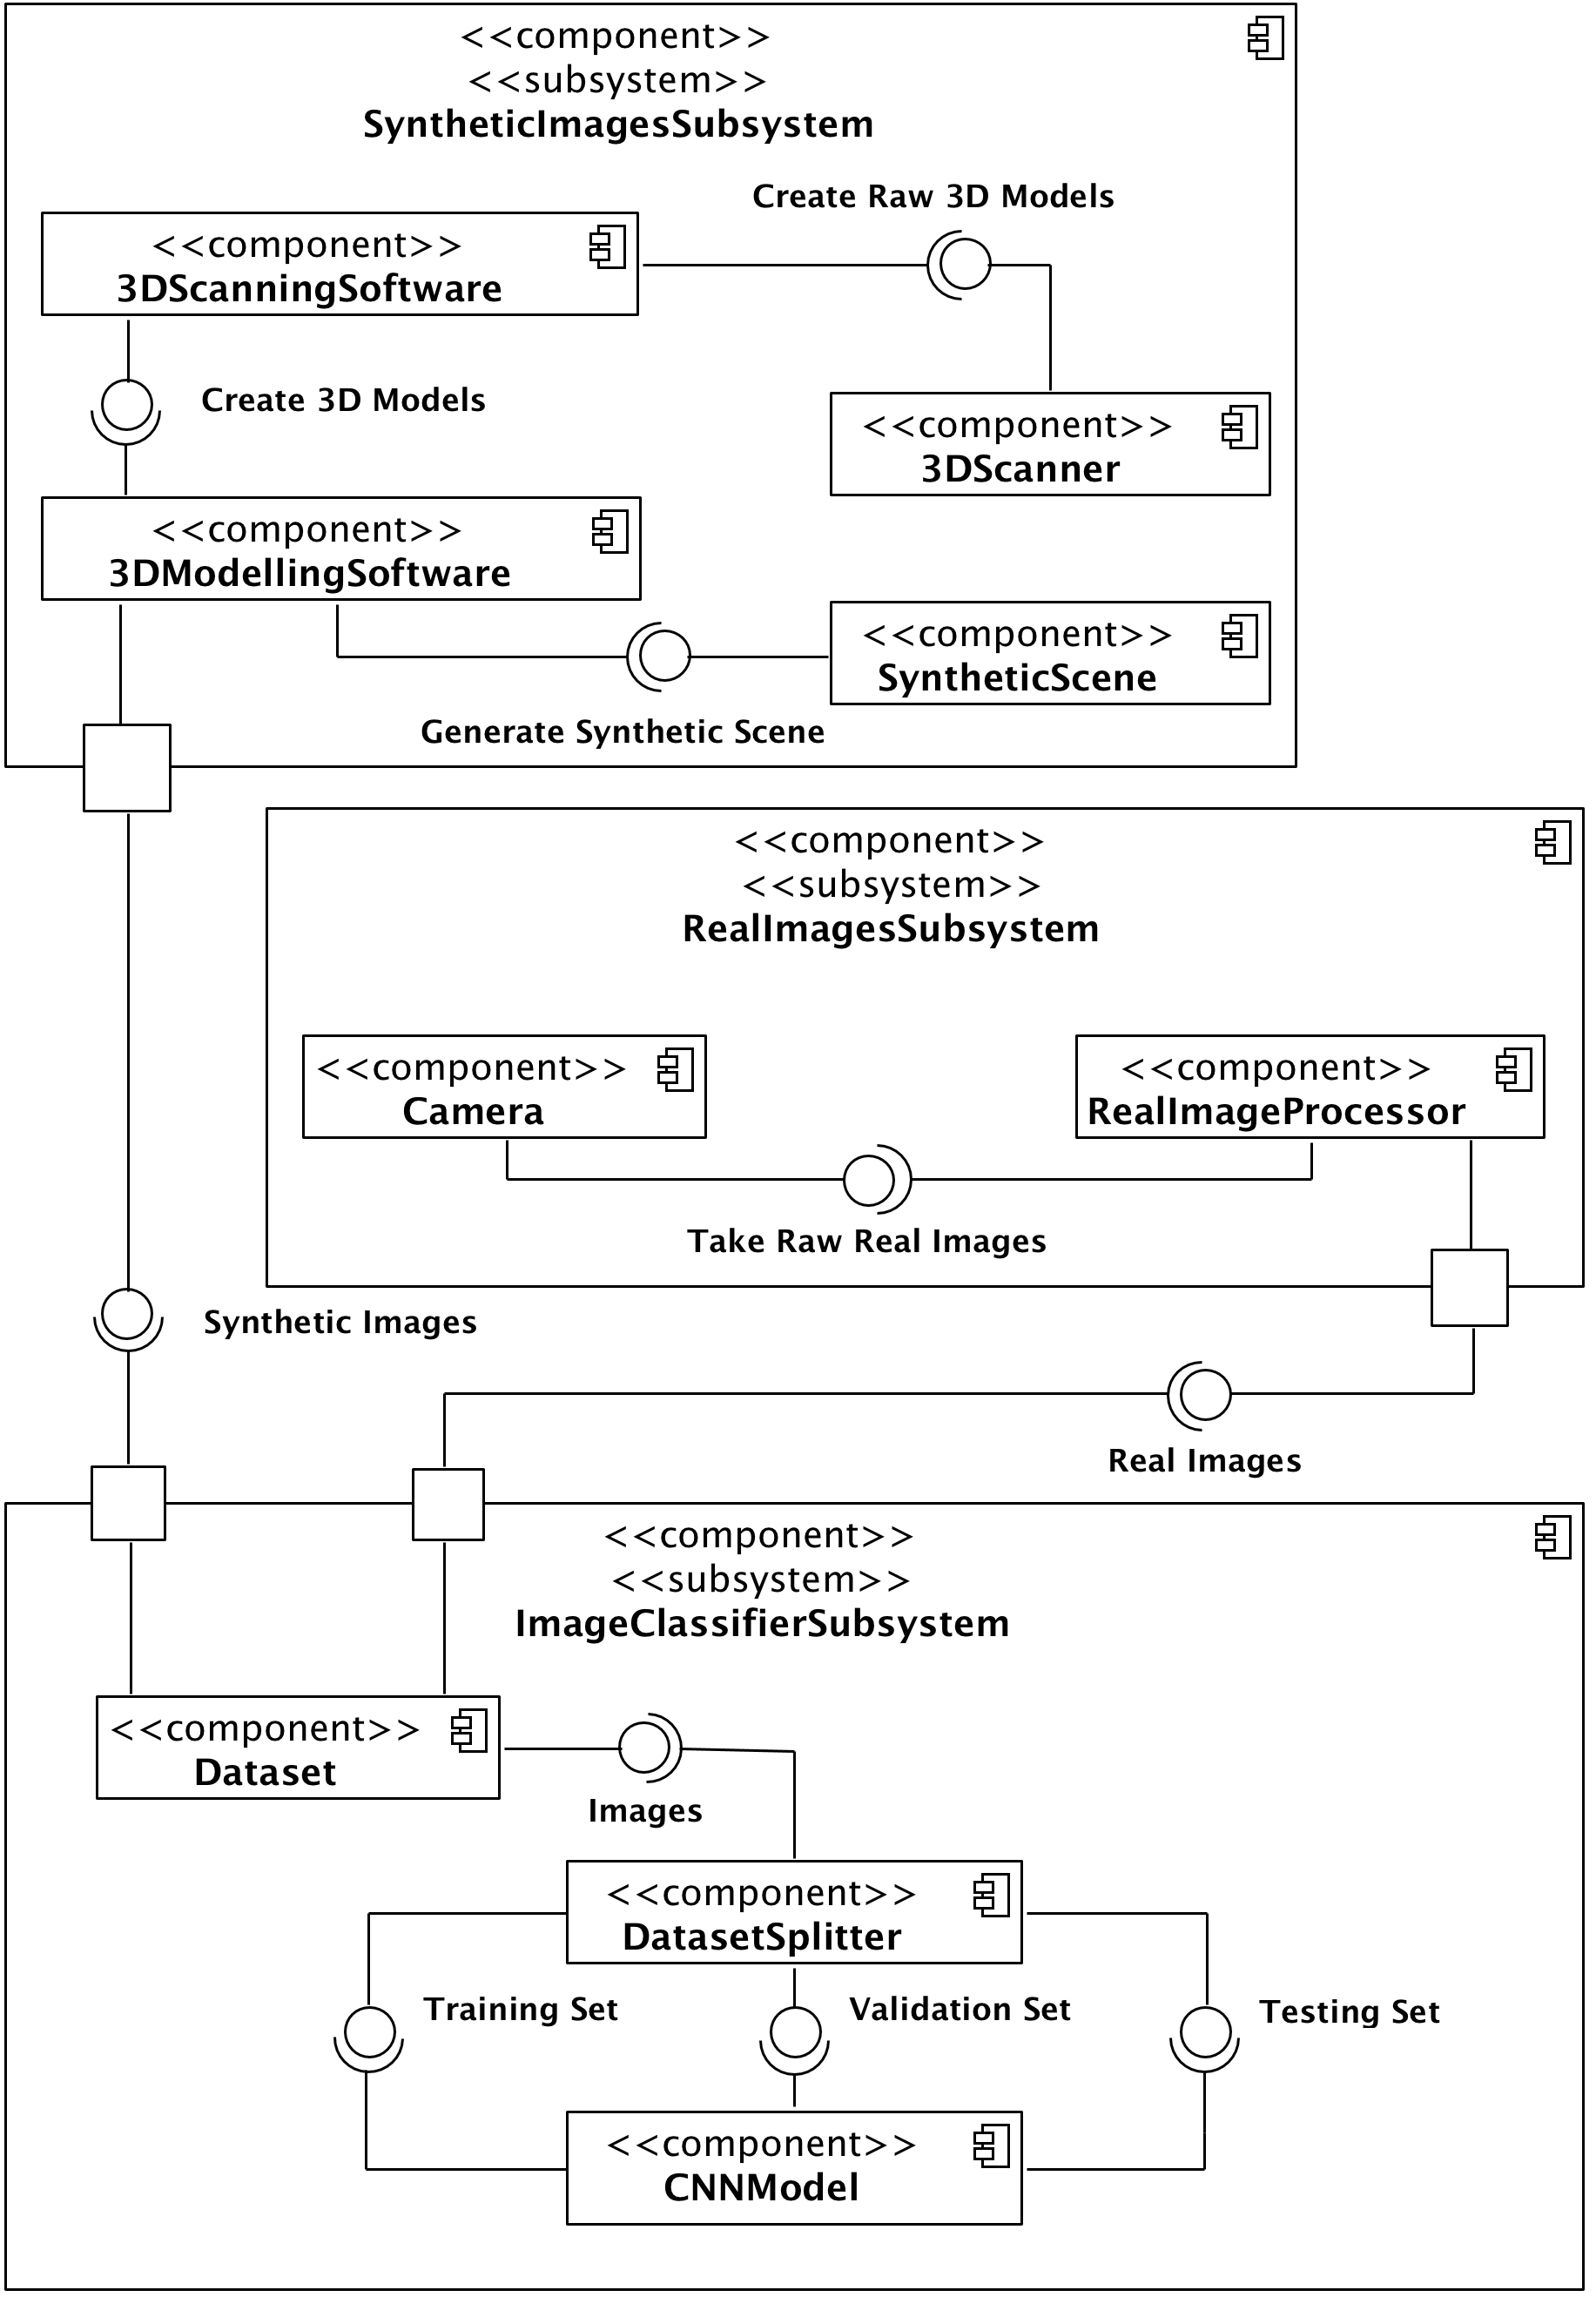
\includegraphics[width=\textwidth]{SSD}
\caption{Subsystem Decomposition}
\label{fig:SSD}
\end{figure}

\section{Hardware Software Mapping}
This section describes how the subsystems are mapped onto existing hardware and software components. Figure [\ref{fig:DD}] depicts the deployment diagram of our system. Our system contains 4 hardware devices: 2 Ubuntu machines, a Windows machine and a Camera.

\begin{figure}[h]
\centering
  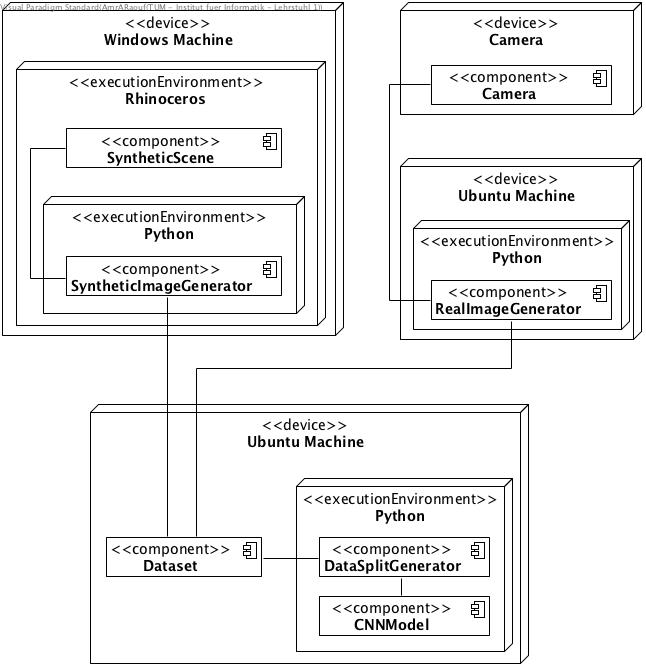
\includegraphics[width=\textwidth]{DD}
\caption{System Deployment Diagram}
\label{fig:DD}
\end{figure}

\subsection{Windows Machine}
The Windows machine is used to run the Rhinoceros 3D modeling software. We chose the windows version of Rhinoceros because it features that are not available on the Ubuntu or Mac versions. We use Rhinoceros to model the SyntheticScene. Moreover, Rhinoceros hosts a python interpreter, which we use to run the SyntheticImageGenerator.

\subsection{Camera}
The Camera is used to capture raw images of the small parts.

\subsection{Ubuntu Machine}
The RealImageGenerator uses the Camera to generate raw real images. The raw real images are then processed by the RealImageGenerator and become ready to be used out of the box.

\subsection{Ubuntu Machine}
The second Ubuntu machine is used to run the ImageClassifier. The Dataset is stored in the Ubuntu machine's file system. We use the system's Python environment to run the DataSplitGenerator and the CNNModel. This Ubuntu Machine is equipped with a Graphics processing unit (GPU). The GPU is used for parallel processing of the Convolutional Neural Network training algorithm. This enhancement significantly slashes down the time needed to train a CNN.

\section{Persistent Data Management}

While our system has no need for a database, the implementation of the ImageClassifier requires the output folder of the DataSplitGenerator to be organized in a certain way. The file structure of the DataSplit is shown in figure [\ref{fig:FS}].

\subsection{DataSplit Root Folder}
The DataSplitGenerator outputs file structure. The root folder contains one folder per small part. Each folder is named after its respective Small Part's label.

\subsection{DataSplit Second Level Folder}
As mentioned above, each Small Part has an assigned folder. This folder, in turn, contains 3 folders: one for training data, one for validation and one for testing.

\subsection{DataSplit Files}
Lastly, each training, validation and testing folder contains a set of images that belong to a specific small part.


\begin{figure}[h]
\centering
  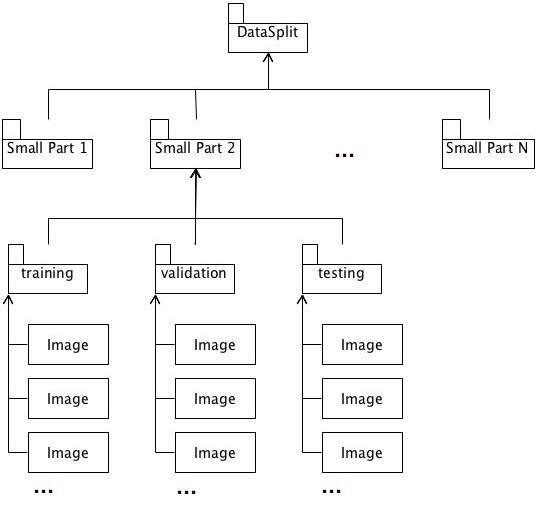
\includegraphics[width=0.8\textwidth]{FS}
\caption{DataSplit File Structure}
\label{fig:FS}
\end{figure}
